% Built from docs/paper/template.tex (CVPR 2026 author kit, https://github.com/cvpr-org/author-kit).
% Build:  cd docs/paper && latexmk -pdf main.tex
\documentclass[10pt,twocolumn,letterpaper]{article}

%%%%%%%%% PAPER TYPE
\usepackage[review]{cvpr}      % layout of the review version; watermark and line numbers removed below      % To produce the REVIEW version

%% This file contains a number of tweaks that are typically applied to the main document.
%% They are not enabled by default, but can be enabled by uncommenting the relevant lines.


%%
%% Official support for 2-column teaser figure
%%
\usepackage{cuted} %< for strip environment

%%
%% For auto-referencing of figures (see fig/teaser.tex and \label{} therein) 
%%
\usepackage{currfile} %< for \currfilebase macro

%%
%% caption and (global) spacing overrides
%%
\usepackage{caption} %< for "\captionof" commands (teaser)
% \setlength{\abovecaptionskip}{.5em} % space above caption
% \setlength{\belowcaptionskip}{1em} % space below caption

%%
%% Inline annotations; for predefined colors, refer to "dvipsnames" in the xcolor package:
%% https://tinyurl.com/overleaf-colors
%%
\newcommand{\red}[1]{{\color{red}#1}}
\newcommand{\todo}[1]{{\color{red}#1}}
\newcommand{\TODO}[1]{\textbf{\color{red}[TODO: #1]}}
%%
%% Disable for camera ready / submission by uncommenting these lines:
%%
% \renewcommand{\TODO}[1]{}
% \renewcommand{\todo}[1]{#1}

%%
%% Work harder in optimizing text layout. Typically shrinks text by 1/6 of page, enable
%% it at the very end of the writing process, when you are just above the page limit.
%%
% \usepackage{microtype}

%%
%% Fine-tune paragraph spacing.
%%
% \renewcommand{\paragraph}[1]{\vspace{.5em}\noindent\textbf{#1.}}

%%
%% Globally adjusts space between figure and caption.
%%
% \setlength{\abovecaptionskip}{.5em}

%%
%% Allows "the use of \paper to refer to the project name"
%% with automatic management of space at the end of the word.
%%
% \usepackage{xspace}
% \newcommand{\paper}{ProjectName\xspace}

%%
%% Commonly used math definitions.
%%
% \DeclareMathOperator*{\argmin}{arg\,min}
% \DeclareMathOperator*{\argmax}{arg\,max}

%%
%% Tighten underline.
%%
% \usepackage{soul}
% \setuldepth{foobar}

%%
%% Reconfigure paragraph (tweaks spacing)
%%

\usepackage{amsmath,amssymb}
\usepackage{booktabs}
\usepackage{graphicx}
\usepackage{xcolor}
\usepackage{tikz}
\usetikzlibrary{arrows.meta,positioning,calc,fit,backgrounds}
\usepackage{microtype}

\definecolor{cvprblue}{rgb}{0.21,0.49,0.74}
\usepackage[pagebackref,breaklinks,colorlinks,allcolors=cvprblue]{hyperref}

\def\paperID{*****}
\def\confName{CVPR}
\def\confYear{2026}

\newcommand{\Aep}{A^{\mathrm{E}}}
\newcommand{\Ast}{A^{\mathrm{S}}}
\newcommand{\gaca}{\textsc{GACA}}

\title{Where Is the Decision Made? Probe-Weighted Token Credit\\for Critic-Free Agent Reinforcement Learning}

\author{Adam Mouedden\\
{\tt\small adam.mouedden@gmail.com}
}

\begin{document}
\ClearShipoutPicture\nolinenumbers  % no CONFIDENTIAL header, CVPR corner marks or line-number ruler
\toggletrue{cvprfinal}  % show the author block instead of "Anonymous submission"
\maketitle
\begin{abstract}
Critic-free reinforcement learning has become the standard way to train language-model agents, but it
assigns credit coarsely: GRPO gives every token of a trajectory the same advantage, and GiGPO and
GACA refine this to the level of an environment step. Inside a step, however, a reasoning model
writes a hundred tokens of chain of thought before a ten-token action, and all of them still share one
advantage. We ask where in that response the decision is actually made. A counterfactual flip test on
ALFWorld (truncate the reasoning, resample the rest, and check whether the action changes) shows that
82\% of the decision is settled before the action is written, that token entropy is a poor guide to
where (the final tenth of a response holds 19\% of the decision but 3\% of the entropy), and that a cheap
teacher-forced \emph{commitment probe}, the measurement behind Causal Importance of Reasoning, tracks
it closely: weighting tokens by the probe's rise places $1.65\times$ more credit on decisive segments
than uniform credit, consistently across task types, held-out games and a trained policy, whereas the
model's own attention from action to reasoning does so only weakly ($1.12\times$). We turn the probe into COMMIT (COMMItment-weighted Token credit), a mean-preserving,
clipped redistribution of each step's GACA advantage over its tokens. In a budget-matched study on
ALFWorld with Qwen2.5-1.5B-Instruct and full fine-tuning (about 6\% of GACA's training budget, same
128 held-out games for every method), COMMIT reaches the highest final success of all
arms (20.3\% against 18.8\% for GACA and 14.1\% for GRPO), but none of the method differences is
statistically resolved at this budget, and a variant that applies the probe to positive advantages only
performs significantly worse than both baselines. We also find that
GACA's per-step criticality score is about 85\% within-state noise. Code, logs and weights are released.
\end{abstract}

\section{Introduction}
\label{sec:intro}

Reinforcement learning from outcome rewards has become the standard recipe for training language
models to reason~\cite{shao2024deepseekmath,guo2025deepseekr1} and, increasingly, to act as agents over
many turns~\cite{feng2025gigpo,wang2025ragen,liang2026gaca}. The dominant algorithms are
\emph{critic-free}: instead of learning a value function, GRPO~\cite{shao2024deepseekmath} samples a
group of trajectories for the same prompt and standardizes each trajectory's return against the group.
The price is coarse credit. In a fifty-step household task every token of every step receives the
same advantage, whether it was the decisive choice of where to look or a routine move along the way.

Two recent methods refine this to the level of an environment step. GiGPO~\cite{feng2025gigpo}
regroups the visits that different rollouts make to the same environment state (an \emph{anchor
state}) and contrasts their discounted returns, which yields a step-level advantage without a critic.
GACA~\cite{liang2026gaca} observes that the right granularity depends on the state and mixes the
episode- and step-level advantages with a per-step weight $\lambda_t$ set by the policy's uncertainty,
the mean token negative log-likelihood (NLL) of the sampled action; it reports 96.9\% success on
ALFWorld at 1.5B parameters, against 86.7\% for GiGPO and 72.8\% for GRPO.

Both methods stop at the step. Yet a modern agent's ``action'' is not a short command: in the
reasoning format these methods are trained with, the model writes roughly a hundred tokens of
chain of thought inside \texttt{<think>} tags and then a ten-token command inside \texttt{<action>}
tags, and every one of those tokens still receives its step's single advantage. If a step was good
because of one sentence of planning, the policy gradient spends most of its credit reinforcing the
boilerplate around it. This paper asks a direct question: \emph{where inside a response is the
decision actually made, and can credit be sent there?}

We answer it in two parts. First, \textbf{measurement}. We run a counterfactual flip test on real
ALFWorld steps: cut the response after $j$ tokens, resample the remainder many times, and record how
often the final action changes. The drop of that flip rate across a segment is the share of the
decision settled inside it. This yields three findings. (i) The decision is made in the reasoning: 82\%
of it is settled before the \texttt{<action>} tag. (ii) Token entropy, the signal behind recent
token-level methods for single-turn reasoning~\cite{wang2025beyond}, does not locate it: the last tenth
of a response carries 19\% of the decision but only 3\% of the entropy, and entropy weighting moves
credit toward decisive segments by only 4\%. (iii) A cheap \emph{commitment probe} does: at each cut,
force the reasoning closed and score the probability of the eventual action under the model. This is
exactly the truncate-and-force measurement that Yu~\etal~\cite{yu2026cir} use to define Causal
Importance of Reasoning (CIR) and that Lanham~\etal~\cite{lanham2023faithfulness} call early
answering. Weighting each token by the probe's rise across its segment places $1.65\times$ more credit
on decisive segments than uniform credit at our training configuration, with the effect consistent
across all six task types, on held-out games, and on a trained policy. Along the way we find that
GACA's own per-step score is about 85\% noise from which reasoning path happened to be sampled.

Second, \textbf{training}. Yu~\etal~use CIR as a scalar bonus in the reward; every token of a response
still shares one advantage. We instead use the probe's per-segment rise to \emph{redistribute} each
step's GACA advantage over the tokens of its response, with weights that are clipped and average to
one, so a step's total credit is unchanged and only where it lands moves
(\cref{fig:method}). The probe costs a teacher-forced scoring pass and no generation. In a study on
ALFWorld with full fine-tuning of Qwen2.5-1.5B-Instruct inside the authors' own training stack
(verl-agent~\cite{feng2025gigpo,sheng2025hybridflow}), with every method evaluated on the same 128
held-out games and compared game by game, probe-weighted credit reaches the highest final success of
any arm. Our budget is about 6\% of GACA's, one seed per arm; at that budget no difference between
methods is statistically resolved, and we report it as such.

\paragraph{Contributions.}
\begin{itemize}\itemsep0pt
\item A counterfactual measurement of where decisions are made inside agent reasoning, and evidence
  that the commitment probe tracks it while entropy and NLL do not and attention only weakly
  does (\cref{sec:measure}).
\item Probe-weighted token credit: a critic-free redistribution of step-level advantage over tokens,
  compatible with GRPO, GiGPO and GACA (\cref{sec:method}).
\item A budget-matched, game-paired comparison of GRPO, GACA and five treatments on ALFWorld, with
  negative results reported (\cref{sec:results}), and a measurement that GACA's criticality score is
  dominated by within-state noise.
\end{itemize}

\begin{figure*}[t]
\centering
\resizebox{\textwidth}{!}{% Method overview: credit at three granularities. Colours follow the paper's palette:
% blue = GRPO/episode, orange = GACA/step, pink = probe/token.
\definecolor{cE}{HTML}{2A78D6}
\definecolor{cS}{HTML}{EB6834}
\definecolor{cP}{HTML}{E87BA4}
\definecolor{cInk}{HTML}{0B0B0B}
\definecolor{cMuted}{HTML}{52514E}
\definecolor{cPanel}{HTML}{F6F6F3}
\begin{tikzpicture}[
  x=1cm, y=1cm,
  tok/.style={minimum width=2.6mm, minimum height=5mm, inner sep=0, draw=white, line width=0.4pt},
  ttl/.style={font=\footnotesize\bfseries, anchor=south west, text=cInk},
  stepl/.style={font=\scriptsize, text=cMuted},
  eq/.style={font=\scriptsize, text=cInk, anchor=north west, align=left},
  panel/.style={fill=cPanel, draw=none, rounded corners=2pt},
]
% ---------------- panel backgrounds
\fill[panel] (-0.15,-1.55) rectangle (5.35,1.55);
\fill[panel] (5.75,-1.55) rectangle (11.25,1.55);
\fill[panel] (11.65,-1.55) rectangle (17.3,1.55);

% ---------------- panel 1: GRPO
\node[ttl] at (0,1.1) {(a) GRPO: one advantage per trajectory};
\foreach \s in {0,1,2} {
  \pgfmathsetmacro{\x}{\s*1.75}
  \foreach \k in {0,...,4} { \node[tok, fill=cE!60] at ({\x+0.13+\k*0.27}, 0.3) {}; }
  \node[stepl] at ({\x+0.67}, -0.15) {step $\s$};
}
\node[eq] at (0,-0.45) {$A_{t,j} = \Aep$ for every step $t$ and token $j$\\
  $\Aep$: trajectory return, standardized in its group};

% ---------------- panel 2: GiGPO / GACA
\begin{scope}[xshift=5.9cm]
\node[ttl] at (0,1.1) {(b) GiGPO / GACA: one advantage per step};
\foreach \s/\sh in {0/25,1/85,2/45} {
  \pgfmathsetmacro{\x}{\s*1.75}
  \foreach \k in {0,...,4} { \node[tok, fill=cS!\sh] at ({\x+0.13+\k*0.27}, 0.3) {}; }
  \node[stepl] at ({\x+0.67}, -0.15) {step $\s$};
}
\node[eq] at (0,-0.45) {$A_t = \lambda_t\,\Ast_t + (1-\lambda_t)\,\Aep$\\
  $\Ast_t$: contrast among visits to the same state\\
  $\lambda_t$: GACA's gate on the response's NLL};
\end{scope}

% ---------------- panel 3: probe-weighted tokens
\begin{scope}[xshift=11.8cm]
\node[ttl] at (0,1.1) {(c) Ours: the step's advantage, spread by the probe};
% one step's response: reasoning tokens then action tokens
\foreach \k/\w in {0/15,1/15,2/18,3/35,4/90,5/95,6/30,7/15,8/15,9/15,10/40,11/40,12/40,13/40} {
  \node[tok, fill=cP!\w] at ({0.13+\k*0.27}, 0.3) {};
}
\draw[cInk, line width=0.5pt] ({0.13+9.5*0.27},0.0) -- ({0.13+9.5*0.27},0.6);
\node[stepl, anchor=north] at (1.35,0.0) {reasoning};
\node[stepl, anchor=north] at (3.3,0.0) {action};
% probe curve q(j), drawn in its own band to the right of the title line
\begin{scope}[shift={(0.13,0.66)}]
  \draw[cMuted, line width=0.3pt] (0,0) -- (3.6,0);
  \draw[cP!80!black, line width=0.8pt] (0,0.04) -- (0.8,0.05) -- (1.1,0.09) -- (1.45,0.17) -- (1.62,0.19) -- (3.6,0.2);
  \node[font=\scriptsize, text=cInk, anchor=west] at (3.62,0.12) {$q(j)$};
\end{scope}
\node[eq] at (0,-0.45) {$A_{t,j} = A_t\, w_{t,j}$,\quad mean$_j\, w_{t,j} = 1$, clipped to $[0.25,4]$\\
  $w_{t,j} \propto q(c_{k+1}) - q(c_k)$ for $j \in [c_k, c_{k+1})$\\
  $q(c) = \pi_\theta(a^\star \mid s_t,\, a_t^{<c},\, \texttt{</think><action>})$};
\end{scope}

% arrows between panels
\draw[-{Stealth[length=2mm]}, cMuted, line width=0.6pt] (5.38,0.3) -- (5.72,0.3);
\draw[-{Stealth[length=2mm]}, cMuted, line width=0.6pt] (11.28,0.3) -- (11.62,0.3);
\end{tikzpicture}
}
\caption{\textbf{Credit at three granularities.} GRPO (left) gives every token of a trajectory one
episode-level advantage. GiGPO and GACA (middle) give each environment step its own advantage, mixing
an anchor-state step contrast $\Ast_t$ with the episode advantage $\Aep$ by a weight $\lambda_t$. All
tokens of the step's response still share it. Probe-weighted credit (right) keeps the step advantage
and redistributes it over the response: the commitment probe $q(j)$ scores how likely the eventual
action is after the first $j$ tokens, and each segment's credit is proportional to how much $q$ rises
across it (weights clipped to $[0.25, 4]$ and renormalized to mean one).}
\label{fig:method}
\end{figure*}

\section{Related Work}
\label{sec:related}

\paragraph{Critic-free RL for language models and agents.}
PPO~\cite{schulman2017ppo} with a learned value function~\cite{schulman2015gae} was the original
workhorse of RL from human feedback~\cite{ouyang2022instructgpt}. GRPO~\cite{shao2024deepseekmath}
removed the critic by standardizing each sampled response's reward against a group of responses to
the same prompt, and with its successors (REINFORCE-style
estimators~\cite{ahmadian2024back}, DAPO's clipping and sampling changes~\cite{yu2025dapo}) it became
the default for reasoning models~\cite{guo2025deepseekr1}. Carrying it to multi-turn agents required
new infrastructure (HybridFlow/verl~\cite{sheng2025hybridflow}, RAGEN~\cite{wang2025ragen}); an
alternative line keeps a critic but makes it hierarchical across turns~\cite{zhou2024archer}.

\paragraph{Step-level credit without a critic.}
GiGPO~\cite{feng2025gigpo} is, to our knowledge, the first critic-free step-level advantage for LLM
agents. It hashes environment states across the group's rollouts into \emph{anchor states} and
standardizes the discounted return of each visit against the other visits to the same state, then
adds this step advantage to the episode one. GACA~\cite{liang2026gaca} argues that the useful
granularity is a property of the state and mixes the two levels with a per-step weight $\lambda_t$
driven by a criticality score, the sampled action's mean token NLL normalized within its trajectory;
it proves that a state-adaptive weight dominates any constant one and that the optimal weight grows
with the anchor-group size. Its Appendix B.4 proposes, but does not train, a leave-one-out score that
averages the NLL of the other visits to the same anchor. Both methods stop at the environment step: all
tokens of a step's response share one advantage. Process reward models~\cite{lightman2024verify,
wang2024mathshepherd} and Monte-Carlo value estimates from intermediate states~\cite{kazemnejad2024vineppo}
offer finer credit at the cost of a learned verifier or many extra rollouts; reward redistribution
methods such as RUDDER~\cite{arjona2019rudder} reshape returns, which reward-shaping theory
constrains~\cite{ng1999shaping}. Our method adds no model and no rollouts.

\paragraph{Token-level signals in RL for reasoning.}
Wang~\etal~\cite{wang2025beyond} show that in single-turn reasoning a small minority of high-entropy
``forking'' tokens drives most of the improvement, and that restricting the policy gradient to them
helps; Cui~\etal~\cite{cui2025entropy} study how RL collapses policy entropy. GACA also scores steps by
uncertainty. We test whether uncertainty locates the \emph{decision} inside an agent's reasoning and
find that it largely does not (\cref{sec:measure}).

\paragraph{Faithfulness and causal importance of reasoning.}
Lanham~\etal~\cite{lanham2023faithfulness} test whether chain of thought is used by truncating it and
forcing an early answer. Bogdan~\etal~\cite{bogdan2025anchors} locate ``thought anchors'', the
sentences that shape a reasoning trace, by resampling the trace from each sentence and, as a white-box
alternative, by inspecting attention between sentences. Yu~\etal~\cite{yu2026cir} formalize the
truncate-and-force measurement as Causal Importance of Reasoning,
$\mathrm{CIR} = \frac{1}{T}\sum_k \mathrm{JS}\big(\mathrm{Bern}(p_k)\,\|\,\mathrm{Bern}(p_T)\big)$
with $p_k$ the probability of the final answer after the first $k$ reasoning tokens, show that outcome
rewards lower it on many tasks, and restore it with a CIR bonus in the reward. Our commitment probe is
this measurement. What we add is its use \emph{inside the advantage}: the probe's per-segment rise
decides which tokens of a step receive that step's credit, in a multi-turn agent, instead of a scalar
bonus shared by all tokens. We also check it against resampling and against attention, the two
signals Bogdan~\etal~compare.

\section{Background: Credit in Critic-Free Agent RL}
\label{sec:background}

\paragraph{Setting.}
An agent interacts with an environment for up to $T$ steps. At step $t$ the policy $\pi_\theta$ reads
a prompt built from the task, recent history and the admissible actions, and emits a response
$a_t = (a_t^1,\dots,a_t^{|a_t|})$: reasoning inside \texttt{<think>} tags followed by a command inside
\texttt{<action>} tags. The environment executes the command; the episode reward is sparse,
$r_T \in \{0, 1\}$ for success, plus a small penalty for malformed responses~\cite{feng2025gigpo}.
For each task a group of $G$ trajectories $\{\tau_i\}_{i=1}^{G}$ is sampled with the same initial state.

\paragraph{Clipped surrogate.}
All methods below share PPO's token-level objective~\cite{schulman2017ppo}
\begin{equation}
\begin{split}
\mathcal{J}(\theta) = \mathbb{E}\Big[\tfrac{1}{|a_t|}\textstyle\sum_{j}
  \min\big(&\rho_{t,j} A_{t,j},\, \mathrm{clip}(\rho_{t,j}, 1\!\pm\!\epsilon)\, A_{t,j}\big)\Big]\\
  &- \beta\, \mathrm{KL}(\pi_\theta \,\|\, \pi_{\mathrm{ref}}),
\end{split}
\label{eq:ppo}
\end{equation}
with $\rho_{t,j}$ the token probability ratio to the sampling policy. They differ only in the
advantage $A_{t,j}$, and until now $A_{t,j}$ has not depended on $j$.

\paragraph{GRPO: episode credit.}
GRPO~\cite{shao2024deepseekmath} standardizes each trajectory's return within its group,
$\Aep_i = (R(\tau_i) - \mu_G)/(\sigma_G + \varepsilon)$, and broadcasts it to every token of every step.

\paragraph{GiGPO: step credit from anchor states.}
GiGPO~\cite{feng2025gigpo} collects every visit, across the group's rollouts, to the same environment
state $z$ (identical observation), forming an anchor group $\mathcal{G}_z$ of size $m_z$. With the
discounted step return $\hat g_t = \sum_{t' \geq t} \gamma^{t'-t} r_{t'}$, the step advantage
standardizes $\hat g_t$ within the anchor group,
$\Ast_t = (\hat g_t - \mu_{\mathcal{G}_z})/(\sigma_{\mathcal{G}_z} + \varepsilon)$
(falling back to prompt-group statistics when $m_z = 1$~\cite{liang2026gaca}), and the two levels are
summed, $A_t = \Aep + w\,\Ast_t$.

\paragraph{GACA: state-adaptive mixing.}
GACA~\cite{liang2026gaca} replaces the sum by a per-step convex mixture
\begin{equation}
A_t = \lambda_t\, w\, \Ast_t + (1 - \lambda_t)\, \Aep.
\label{eq:gaca}
\end{equation}
The weight comes from a criticality score: the mean token NLL of the sampled response,
$H_t = -\frac{1}{|a_t|}\sum_j \log \pi_{\theta_{\mathrm{old}}}(a_t^j \mid s_t, a_t^{<j})$, normalized by its
trajectory mean, $c_t = H_t / \bar H$. A piecewise-linear gate maps it to the weight,
$\lambda_t = \lambda_0(1 + \alpha(c_t - 1))$ for $c_t \geq 1$ and $\lambda_0(1 - \beta(1 - c_t))$
otherwise, clamped to $[0, 1]$, with $\lambda_0 = 0.5$ and $\alpha = \beta = 0.5$. Uncertain steps
lean on the step contrast, confident steps on the episode return. GACA's analysis gives the
MSE-optimal weight as $\lambda^\star_z = M_E/(M_E + M_S)$, the ratio of the two estimators' errors, and
shows it is non-decreasing in $m_z$; the NLL enters as a one-sided certificate of local decision
criticality. In every case above, all $|a_t|$ tokens of a response share $A_t$.

\section{Probe-Weighted Token Credit}
\label{sec:method}

\paragraph{The commitment probe.}
Let $a^\star$ be the command the response eventually issued and $c$ a cut point in the response. The
probe asks how strongly the reasoning written so far commits the model to $a^\star$:
\begin{equation}
q(c) = \pi_\theta\big(a^\star \,\big|\, s_t,\; a_t^{<c},\; \texttt{</think><action>}\big),
\label{eq:probe}
\end{equation}
the probability of the original command's tokens when the reasoning is cut after $c$ tokens and
closed by force. It needs one teacher-forced forward pass per cut and no sampling. This is the
quantity $p_k$ of CIR~\cite{yu2026cir} and the early-answering test of~\cite{lanham2023faithfulness};
$q(0)$ is the probability of the eventual action before any reasoning, and $q$ reaches one by
construction once the command is written.

\paragraph{From probe to token weights.}
We place cuts $0 = c_0 < c_1 < \dots < c_K$ every 16 reasoning tokens and at the start of the
\texttt{<action>} tag, and treat the response end $L$ as a final cut with $q = 1$. Segment $k$, the
tokens $[c_k, c_{k+1})$, receives the rise of the probe across it, spread evenly over its tokens:
\begin{equation}
\tilde w_j = \frac{\max\big(q(c_{k+1}) - q(c_k),\, 0\big)}{c_{k+1} - c_k}, \qquad j \in [c_k, c_{k+1}).
\label{eq:raw}
\end{equation}
The raw weights are normalized to mean one over the response, clipped to $[0.25, 4]$ and renormalized,
iterating to a fixed point. The step's token advantages are then
\begin{equation}
A_{t,j} = A_t \cdot w_{t,j}, \qquad \tfrac{1}{|a_t|}\textstyle\sum_j w_{t,j} = 1,
\label{eq:ours}
\end{equation}
with $A_t$ from GACA (\cref{eq:gaca}). Because the weights average one, the length-normalized
contribution of each step in \cref{eq:ppo} is unchanged; only where the credit lands inside the response
moves. A flat probe (the action was certain from the start) gives uniform weights, recovering GACA
exactly, and malformed responses with no action keep uniform weights.

\paragraph{What it does and does not change.}
Rollouts, the importance ratio and the KL term are untouched, so training stays on-policy; the probe
only decides how much each token's gradient counts, much as a fixed reward model would. It says
\emph{where} a step's decision was made, not whether the decision was good, which remains the job of
$A_t$. A good step therefore reinforces mostly the reasoning that produced its action, and a bad step
penalizes mostly that reasoning rather than the surrounding boilerplate. Under the assumption that a
step's value flows through its action, which holds in ALFWorld where only the command touches the
environment, $A_t w_{t,j}$ approximates each token's causal contribution to the step's value. The
method is orthogonal to the step estimator and applies to GRPO or GiGPO advantages unchanged.

\paragraph{Cost.}
With cuts every 16 tokens a $\sim$95-token response needs about seven scoring passes over prompts of
$\sim$500 tokens, computed in the same batched routine that recomputes the old-policy log-probabilities.
In our runs this added about 150\,s to a $\sim$390\,s iteration (\cref{sec:results}); generation is
unaffected and inference uses no probe at all.

\paragraph{Variants.}
We test three ways of applying the probe, each motivated by a failure mode of concentrating credit:
\emph{(i)} a tighter clip $[0.5, 2]$, in case large weights make updates too big;
\emph{(ii)} probe weights only where $A_t > 0$, in case a wrong-signed advantage concentrated on the
decisive reasoning is especially harmful at low success rates; and \emph{(iii)} scoring the probe with
the frozen reference policy instead of the current one, to break a possible feedback loop in which the
policy grades its own reasoning and credit for early commitment pushes the decision earlier, the
pattern~\cite{yu2026cir} report for outcome rewards. We also evaluate two step-level changes to GACA
that target its estimator's reliability rather than tokens: scaling the gate's odds by
$1 - 1/m_z$ (GACA's own analysis says $\lambda^\star$ grows with $m_z$, but $m_z$ never enters its gate;
a singleton anchor group gets $\lambda_t = 0$) and the leave-one-out score of GACA's Appendix B.4.

\section{Experimental Setup}
\label{sec:setup}

\paragraph{Benchmark and model.}
We use ALFWorld~\cite{shridhar2020alfworld}, the text household benchmark on which GACA reports its
ablations, with all six task types (pick-and-place, examine in light, clean, heat, cool, and pick two)
and a 50-step horizon. The policy is Qwen2.5-1.5B-Instruct~\cite{qwen2025qwen25}, the paper's smaller
scale, fully fine-tuned. Training runs in verl-agent~\cite{feng2025gigpo,sheng2025hybridflow}, the
stack GACA builds on, with the authors' ALFWorld prompt (ReAct-style~\cite{yao2022react} reasoning in
\texttt{<think>} tags, a command in \texttt{<action>} tags, 512-token responses, a two-step history) and
vLLM~\cite{kwon2023vllm} rollouts. Each method is a different advantage estimator plugged into the
same trainer; GRPO, GACA and all treatments call one shared, unit-tested implementation.

\paragraph{Recipe and budget.}
We keep GACA's shared configuration: group size 8, learning rate $10^{-6}$, $\gamma = 0.95$, KL
coefficient 0.01 with the low-variance estimator, invalid-format penalty 0.1, mean-and-std
normalization, $\lambda_0 = 0.5$, $\alpha = \beta = 0.5$. The budget is the one deliberate difference
(\cref{sec:budget}): on a single A100 40\,GB we train 4 tasks $\times$ 8 rollouts for a fixed 34
iterations, 1,088 trajectories per method, about 6\% of the published 19,200. All curves are still
rising at the end, so the comparison is of early learning at a matched rollout budget, and our absolute
success rates are not comparable to published ones.

\paragraph{Evaluation.}
Every method is evaluated every 10 iterations and at the end on the \emph{same} 128 held-out games
(ALFWorld's in-distribution validation split, one episode each, sampling temperature 0.4 as in the
authors' recipe). Because the games are shared, two methods are compared game by game with an exact
McNemar test~\cite{mcnemar1947} on the games one method solves and the other does not, which is far
more sensitive than comparing two rates at $n = 128$. We report the final checkpoint; the paper's
best-checkpoint convention picks the maximum of several noisy evaluations and is optimistic. One game
is 0.78 points. The base model solves 6 of 128 (4.7\%).

\paragraph{Methods.}
The controls are GRPO and GACA. The treatments are GACA with the $m_z$ reliability gate, GACA with the
leave-one-out score (GACA-LOO), COMMIT applied to GACA's step advantage, and two COMMIT variants
(\cref{sec:method}). One seed per method; the probe arm used a different training-environment seed
(the order in which training games are drawn) than the other arms, with the evaluation games pinned to
be identical. In an earlier pilot of this project, two seeds of the same method differed by 3.1 points at a matched
checkpoint, so differences of a few points between single runs are within seed noise.

\section{Where Is the Decision Made?}
\label{sec:measure}

Before training, we measure. All studies in this section use no training and run on real steps
sampled by the policy in the format above.

\subsection{GACA's step score is mostly path noise}
\label{sec:noise}
GACA's gate reads the mean NLL of the one response that was sampled. Exact token entropy,
$-\sum_v \pi(v)\log\pi(v)$ over the vocabulary, is available from the same forward pass and does not
depend on which token was drawn, so it removes the single-sample noise of the NLL at each position. On
7,864 step rows from the first five iterations of a GACA-family run, the two scores agree almost
perfectly (Pearson 0.94, within-trajectory Spearman 0.90): replacing NLL by exact entropy moves
$\lambda_t$ by more than 0.1 on only 0.9\% of steps. Averaging over $\sim$95 tokens already cancels
token-level sampling noise. The noise that remains is of another kind. At anchor states visited at
least twice in a group (575 states), visits to the \emph{same} state differ only in which reasoning
path was sampled, and that within-state variation accounts for 87\% of the variance of the NLL score
(85\% for exact entropy). GACA's criticality score is therefore mostly a property of the sampled path,
not of the state whose criticality it is meant to certify, which may explain why the paper's own
random-permutation control is needed to show that the gate's placement matters. Averaging across visits
(GACA-LOO) removes this noise but also the per-visit contrast; we test it in \cref{sec:results}.

\subsection{A counterfactual flip test}
To find where a decision is made inside a response, we intervene on it. For a step with response of
$L$ tokens and issued command $a^\star$, we cut the response after $j$ tokens at about 18 points
(every $L/16$ tokens plus the \texttt{<action>} tag), resample the remainder 8 times at temperature 1,
and record $F(j)$, the fraction of continuations whose command differs from $a^\star$. $F$ falls from
$F(0)$ (resample everything) to $F(L) = 0$, and its drop across a segment,
$F(c_k) - F(c_{k+1})$, is the share of the decision settled inside it. Because ALFWorld is
deterministic, an unchanged command implies an identical next state, so this is an exact step-level
relevance measure. We sample 320 valid steps from base-policy rollouts on 48 training games, which costs
44k continuations and about five minutes on one GPU with vLLM. The study is run twice on disjoint game
sets: once to design weighting schemes and once held out to test them.

Decisions are genuinely open and are made in the reasoning. Resampling a whole response changes the
command 72\% of the time, and 82\% of the decision mass is settled before the \texttt{<action>} tag.
\Cref{fig:deciles} shows where. Decision importance is spread through the reasoning and peaks in its
last tenth, where the model commits (18.8\%). Entropy follows a different profile: it is high in the
middle of the reasoning and lowest at the end (2.8\%), because once the model has committed, the tokens
that express the commitment look certain.

\begin{figure}[t]
\centering
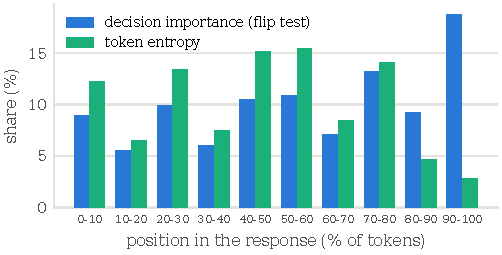
\includegraphics[width=\linewidth]{figs/deciles.pdf}
\caption{\textbf{Where the decision is made vs.\ where the entropy is}, by position in the response
(held-out flip test, 320 steps). The final tenth of a response holds 18.8\% of the decision but 2.8\%
of the token entropy.}
\label{fig:deciles}
\end{figure}

\subsection{Which signal locates the decision?}
We score each token-weighting scheme by the share of its credit that lands on decision importance,
$\sum_k m_k\, d_k$ for credit shares $m_k$ and importance shares $d_k$ over the fine flip-test segments,
relative to uniform credit (GACA), and by total-variation distance to importance. \Cref{fig:oracle}
summarizes. Token entropy, the signal behind single-turn ``forking token''
methods~\cite{wang2025beyond}, moves credit toward decisive segments by only 2--4\% and fits importance
\emph{worse} than uniform (TV $+0.011$, 95\% CI $[+0.003, +0.018]$). Sampled NLL does no better, and a
fixed $2\times$ weight on the action tokens gives 4--5\%. A hybrid designed on the first run (entropy on
the reasoning, protected action tokens) did not hold out of sample (1.07$\times$). The commitment probe
is the only scheme that fits importance better than uniform: its unclipped segment weights put
$2.94\times$ more credit on decisive segments (TV $-0.065$, CI $[-0.093, -0.037]$).

\begin{figure}[t]
\centering
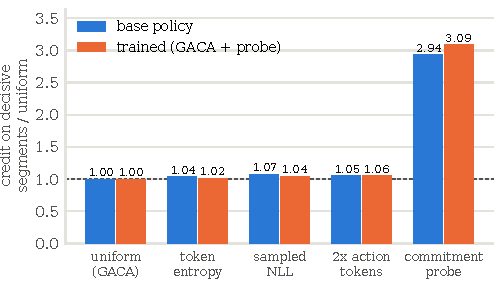
\includegraphics[width=\linewidth]{figs/oracle.pdf}
\caption{\textbf{Credit on decisive segments relative to uniform credit}, by weighting scheme, on held-out
games, for the base policy and for the final policy of the COMMIT training run. Unclipped
segment weights; the clipped training configuration gives $1.65\times$ and $1.64\times$.}
\label{fig:oracle}
\end{figure}

\paragraph{Robustness at the training configuration.}
\Cref{fig:robust} evaluates the exact function used in training (clip $[0.25, 4]$, mean-preserving). It
gives $1.65\times$ (CI $[1.57, 1.74]$) and beats uniform on 80\% of steps. The effect holds for every
task type ($1.52$ to $1.96\times$), for both halves of the games (1.73 and 1.57), for early and late steps,
and with cuts up to three times coarser (1.53). It is largest where it matters most, on steps whose
decision was open ($2.37\times$ against $1.33\times$ when settled). The clip trades concentration for
stability: unclipped weights give $2.18\times$, a $[0.5, 2]$ clip $1.26\times$.

\begin{figure}[t]
\centering
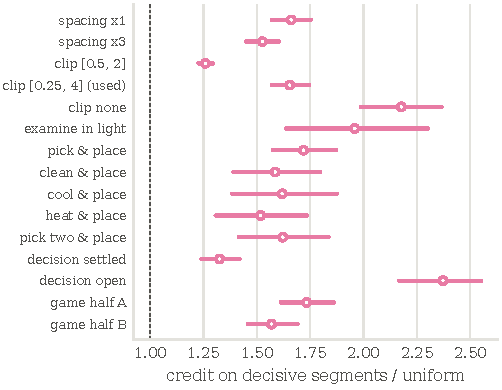
\includegraphics[width=\linewidth]{figs/robust.pdf}
\caption{\textbf{Robustness of probe weights} at the training configuration: credit on decisive
segments relative to uniform with 95\% bootstrap intervals, by cut spacing, clip, task type, decision
openness and game half.}
\label{fig:robust}
\end{figure}

\subsection{Does attention locate it?}
\label{sec:attention}
Bogdan~\etal~\cite{bogdan2025anchors} use attention between sentences as a white-box alternative to
resampling. A transformer computes, for each query token, a softmax-normalized distribution over
earlier keys, $\mathrm{softmax}(QK^\top/\sqrt{d})$~\cite{vaswani2017attention}. We read the attention
that the command tokens pay to each reasoning token, averaged over heads and over the last third of
the layers, and score it like a weighting scheme on 128 held-out steps, restricted to the reasoning
segments (where attention is defined) and compared with the probe on the same segments. Attention does
point toward the decision, but weakly: it places $1.12\times$ more credit on decisive segments than
uniform (CI $[1.03, 1.24]$), against $1.61\times$ ($[1.45, 1.77]$) for the probe on the same steps, and
its per-step rank correlation with importance density is only 0.14. \Cref{fig:example} shows why on
one step. More than half of the decision is settled in the single segment ``\emph{[let's check] the
drawers to see if any have}'', which commits the agent to searching the drawers before it writes
\texttt{go to drawer 1}. The probe puts its weight there. Attention is diffuse and peaks on the
tokens just before the action tag, which is consistent with the view that attention weights are not, by
themselves, explanations~\cite{jain2019attention}.

\begin{figure*}[t]
\centering
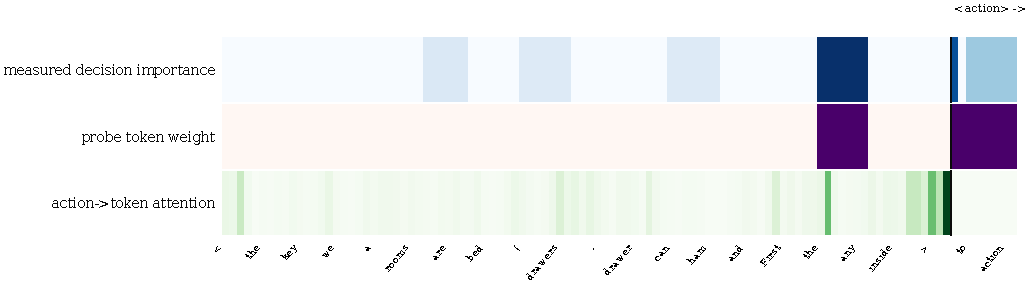
\includegraphics[width=\linewidth]{figs/example.pdf}
\caption{\textbf{One held-out step, token by token.} Top: decision importance measured by the flip
test (darker = more of the decision settled there). Middle: COMMIT credit. Bottom: attention
from the command tokens to each reasoning token (last third of the layers, mean over heads). The
vertical line marks the \texttt{<action>} tag. The task is to put a keychain on a desk; before any
reasoning the eventual command has probability $q(0) = 0.04$ and resampling the whole response changes
it 75\% of the time. 53\% of the decision is settled in one segment, ``the drawers to see if any
have'', where the probe also concentrates its weight; attention is spread out and peaks next to the
action tag.}
\label{fig:example}
\end{figure*}

\subsection{The probe survives training}
The flip test above uses the base policy. Repeating it on the same held-out games with the final weights
of our COMMIT training run gives the same picture: the probe's credit on decisive segments is
$1.64\times$ at the training configuration (CI $[1.55, 1.72]$; base model $1.65\times$) and $3.09\times$
unclipped, entropy stays near $1\times$, and the share of the decision inside the action tags moves only
from 18\% to 21\%. Training does not degrade the probe as a measurement of where decisions are made.

\section{Training Results}
\label{sec:results}

\Cref{tab:results} lists the final held-out success of every method together with paired comparisons
against both controls, and \cref{fig:curves} shows the learning curves.

\begin{table}[t]
\centering\footnotesize
\setlength{\tabcolsep}{3.2pt}
\begin{tabular}{@{}lrrcc@{}}
\toprule
Method & Final & Best & vs.\ GRPO & vs.\ GACA \\
\midrule
Base model (no training) & 4.7 & -- & -- & -- \\
GRPO~\cite{shao2024deepseekmath} & 14.1 & 14.1 & -- & 13/7 (0.26) \\
GACA~\cite{liang2026gaca} & 18.8 & 18.8 & 7/13 (0.26) & -- \\
\midrule
GACA + $m_z$ gate & 12.5 & 12.5 & 13/11 (0.84) & 17/9 (0.17) \\
GACA-LOO (App.~B.4 of~\cite{liang2026gaca}) & 11.7 & 11.7 & 11/8 (0.65) & 14/5 (0.064) \\
\textbf{COMMIT (ours)} & 20.3 & 20.3 & 8/16 (0.15) & 14/16 (0.86) \\
\quad clip $[0.5, 2]$ & 14.1 & 14.1 & 13/13 (1.00) & 16/10 (0.33) \\
\quad positive $A_t$ only & 5.5 & 6.2 & \textbf{16/5 (0.027)} & \textbf{20/3 (<0.001)} \\
\bottomrule
\end{tabular}

\caption{\textbf{Held-out success (\%) on the same 128 ALFWorld games}, 34 training iterations
(33 for the two GACA step variants), one seed per method. \emph{Final} is the end-of-training
checkpoint, \emph{Best} the maximum over five evaluations. The comparison columns give $b/c$
(McNemar $p$): $b$ games solved only by the control, $c$ only by the method in that row; bold
$p < 0.05$.}
\label{tab:results}
\end{table}

\begin{figure}[t]
\centering
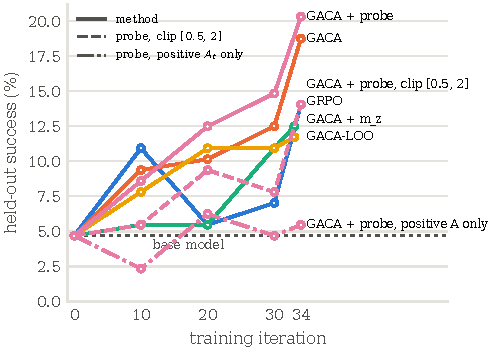
\includegraphics[width=\linewidth]{figs/curves.pdf}
\caption{\textbf{Held-out success over training} (128 games, evaluated every 10 iterations). Colour
follows the method; variants of the probe keep its colour and change line style.}
\label{fig:curves}
\end{figure}

\paragraph{Controls.}
Both controls learn: GRPO reaches 14.1\% and GACA 18.8\% from the base model's 4.7\% (both $p < 0.05$
against the base model, game-paired). GACA leads GRPO by 13 games to 7
($p = 0.26$): at this budget the ordering is not resolved. GACA's gate is active in our runs: the
criticality score has standard deviation 0.35 and $\lambda_t$ has standard deviation 0.087, so steps do
receive different mixtures.

\paragraph{Probe-weighted token credit.}
GACA + probe reaches 20.3\%, the highest final success of any method, after rising at every evaluation
(4.7, 8.6, 12.5, 14.8, 20.3) and leading every arm from iteration 20 on. It also has the highest
training-batch success (11.2\% averaged over iterations, against 9.2\% for GACA). Game by game it solves
16 games GACA misses while missing 14 that GACA solves ($p = 0.86$), and against GRPO the split is 16 to
8 ($p = 0.15$). We read this as \emph{consistent with} a benefit, not as evidence for one: with one seed
per arm and a 3-point seed-to-seed spread observed earlier, a 1.5-point lead over GACA is well within
noise. The probe's cost is visible in wall-clock: 550\,s per iteration against 389\,s for GACA, of which
151\,s is the probe passes. Its updates are moderately larger than GACA's (mean gradient norm 1.06
against 0.84, KL 0.024 against 0.020), as expected when the same advantage is concentrated on fewer
tokens. The probability of the eventual action before any reasoning, $q(0)$, \emph{fell} from 0.19 to
0.14 over training, so the reasoning became more causally important rather than decorative, the
opposite of the drift Yu~\etal~\cite{yu2026cir} warn about for outcome rewards.

\paragraph{How the probe is applied matters.}
The two variants were designed to fix failure modes of concentration, and none helped.
A tighter clip $[0.5, 2]$ brought the gradient norm to GACA's level (0.93) and finished at 14.1\%, level
with GRPO. Applying the probe only to positive advantages, so that blame always stays uniform, was the
worst method: 5.5\%, essentially no learning, and significantly below both GRPO (16 to 5, $p = 0.027$)
and GACA (20 to 3, $p < 0.001$). Its KL rose to 0.059 over the last iterations although $q(0)$ stayed flat
(0.20 to 0.19), so early commitment does not explain the failure. A plausible reading is that the
asymmetry itself is harmful: positive steps push hard on a few decisive tokens while negative steps push
weakly on all tokens, so the policy is moved toward specific reasoning patterns without a matching
signal moving it away from bad ones.

\paragraph{Step-level treatments.}
Neither change to GACA's step estimator helped. Scaling the gate's odds by $1 - 1/m_z$ changes little
because 96\% of steps already fall in anchor groups with $m_z \geq 2$; it finished at 12.5\%. The
leave-one-out score of GACA's Appendix B.4, which averages away the within-state noise we measured,
finished at 11.7\% and trails GACA by 14 games to 5 ($p = 0.064$). Pooling the score also shrinks the
spread of $\lambda_t$ to 0.039 from 0.087, so the gate barely adapts; in the paper's terms, it trades the
noise of the single-sample score for the loss of within-group resolution, and at this budget the trade
does not pay.

\section{Discussion and Limitations}
\label{sec:discussion}

\paragraph{What the evidence supports.}
The measurement results are the firm part of this paper. They are counterfactual, repeated on disjoint
game sets and on a trained policy, and come with intervals. Inside an agent's reasoning the decision is
made before the command is written; uncertainty signals (entropy, NLL) do not locate it; the commitment
probe does. GACA's criticality score is dominated by within-state path noise. The training results are
weaker. Probe-weighted credit had the highest final success, and the variants that changed how it is
applied did worse, two of them significantly. With one seed per arm and about 6\% of the published
training budget, no difference between the main methods is statistically resolved.

\paragraph{Why a better measurement need not train better.}
The probe changes where credit lands, not whether it is right. At 5--15\% training success most step
advantages rest on one or two successful rollouts in a group of eight, so their sign is often wrong;
concentrating a wrong-signed advantage on the reasoning that produced the decision does more damage than
spreading it. Uniform credit is, in this sense, a hedge against a noisy step estimator, and the positive-
only variant shows that asymmetric hedging is worse than none. We expect probe weighting to pay off more
where step advantages are reliable: at higher success rates, with more rollouts per group, or combined
with an estimator that scales concentration by its own confidence, for instance the number of successful
rollouts in the group or whether the anchor group carries a real return contrast.

\paragraph{Limitations.}
\emph{Budget and seeds}: about 6\% of GACA's trajectories and one seed per method, so method
differences of a few points are not interpretable on their own; the paired tests are the right lens,
and they are mostly inconclusive. \emph{Training seed}: the probe arm drew its training games in a
different order than the controls, with identical evaluation games. \emph{Benchmark}: ALFWorld only;
WebShop, the paper's second benchmark, needs a product-search server we did not stand up.
\emph{Oracle}: the flip test measures relevance for the next command only, not for the episode's
outcome, and uses 8 resamples per cut; importance is a difference of two noisy rates. \emph{Probe}: as a
likelihood ratio under teacher forcing, the probe can credit a segment that makes the eventual command
\emph{expressible} rather than one that decides it. \emph{Cost}: the probe adds about 40\% to an iteration
in our setup; computing it from a prefix-shared batch would reduce this.

\paragraph{Outlook.}
The cheapest next steps follow directly: multiple seeds of the probe and GACA at this budget, the
paper's 16-task batch, and probe weights scaled by a confidence in the step advantage. More broadly, our
results suggest a separation of concerns for critic-free agent RL: the step estimator decides
\emph{how much} credit a step earns, and a counterfactual probe decides \emph{which tokens} earned it.
The second is now cheap and measurable; the first is the bottleneck.

\section{Conclusion}
We asked where, inside an agent's reasoning, the decision is made. A counterfactual flip test answers
that it is made in the reasoning, mostly not where the model is uncertain, and that a teacher-forced
commitment probe, the measurement behind CIR, finds it reliably. We turned the probe into a
mean-preserving redistribution of GACA's step advantage over tokens. In a budget-matched, game-paired
study on ALFWorld it achieved the best final success of the methods we trained, but the margins are
within single-seed noise, and ways of applying it that seemed safer did worse. Measuring where credit
belongs has become easy; making the credit itself reliable is the open problem.

{
    \small
    \bibliographystyle{ieeenat_fullname}
    \bibliography{main}
}
\end{document}
